\documentclass{article}

% if you need to pass options to natbib, use, e.g.:
%     \PassOptionsToPackage{numbers, compress}{natbib}
% before loading neurips_2018

% ready for submission
% \usepackage{neurips_2018}

% to compile a preprint version, e.g., for submission to arXiv, add add the
% [preprint] option:
%     \usepackage[preprint]{neurips_2018}

% to compile a camera-ready version, add the [final] option, e.g.:
     \usepackage[final]{nips_2018}

% to avoid loading the natbib package, add option nonatbib:
%     \usepackage[nonatbib]{neurips_2018}

\usepackage[utf8]{inputenc} % allow utf-8 input
\usepackage[T1]{fontenc}    % use 8-bit T1 fonts
\usepackage{hyperref}       % hyperlinks
\usepackage{url}            % simple URL typesetting
\usepackage{booktabs}       % professional-quality tables
\usepackage{amsfonts}       % blackboard math symbols
\usepackage{nicefrac}       % compact symbols for 1/2, etc.
\usepackage{microtype}      % microtypography
\usepackage{graphicx}
\usepackage{placeins}
\usepackage[german]{babel}
\usepackage{xcolor}

\title{DLM Semesterprojekt: Bestimmung der 3D-Boundingbox eines Roboters}

% The \author macro works with any number of authors. There are two commands
% used to separate the names and addresses of multiple authors: \And and \AND.
%
% Using \And between authors leaves it to LaTeX to determine where to break the
% lines. Using \AND forces a line break at that point. So, if LaTeX puts 3 of 4
% authors names on the first line, and the last on the second line, try using
% \AND instead of \And before the third author name.

\author{%
  GruppeNR: 1, Namen: Tim Eisenacher (1870755) und Paul Manea(1870391) \\
  EMail: 1870755@stud.hs-mannheim.de
  % examples of more authors
  % \And
  % Coauthor \\
  % Affiliation \\
  % Address \\
  % \texttt{email} \\
  % \AND
  % Coauthor \\
  % Affiliation \\
  % Address \\
  % \texttt{email} \\
  % \And
  % Coauthor \\
  % Affiliation \\
  % Address \\
  % \texttt{email} \\
  % \And
  % Coauthor \\
  % Affiliation \\
  % Address \\
  % \texttt{email} \\
}

\begin{document}
% \nipsfinalcopy is no longer used

\maketitle


\begin{abstract}
The motivation of this project is the 3D bounding box estimation of a roboter using deep learning algorithms. Large groups of patients can benefit from the great potential of modern computer vision , for example in radiological diagnostics or in  automated surgery. Due to increasingly high-resolution images and increasing data volumes, Convolutional Neural Networks (CNN) are particularly well suited to solve this problem due to their high performance. Therefore, the YOLO (You Only Look Once) network architecture as a state of the art real-time object detection system is introduced in this work. With small architectural modifications and a custom loss function, YOLO's high performance and accuracy in solving the problems of this work can be demonstrated. For this purpose, the object recognition was first implemented for a 2D problem and then extended to recognize the robot in a 3D to 2D projection. All in all it is determined that the 3D bounding box estimation can significantly benefit from
using YOLO as a fast and accurate bounding box regression system. Also the YOLO implementation is well suited for real-time image processing.	
\end{abstract}

\newpage
\section{Einleitung}

Objekterkennung ist einer der vielversprechendsten und am stärksten im Forschungsfokus stehenden Bereiche von \textit{Computer Vision} und \textit{Machine Learning} \cite{Ouyang2014}. Besonders im Bereich der medizinischen und industriellen Innovationen konnten dadurch bereits jetzt schon große Fortschritte erzielt werden  \cite{Tremblay1809, Abstract2016}. So können beispielhaft Operationsroboter stark von einer auf \textit{Deep-Learning}-Algorithmen basierenden Erkennung und Lokalisation der Operationsinstrumente profitieren \cite{Surgery1803}. Auch in der Tumordiagnostik kann so die Erkennungsgenauigkeit gegenüber einer menschlichen Klassifikation bei gleichzeitig signifikant niedrigeren Kosten verbessert werden \cite{Cruz-Roa2017}.\newline
Die Anforderungen an die Bildverarbeitung sind dabei in diesen Bereichen besonders groß. Zum einen sorgen immer hochauflösendere Bilder für enorme Datenmengen und damit auch für höhere Hardwareanforderungen. Zum anderen ist die Anzahl an möglichen Klassen und damit Featurekombinationen bei der Objekterkennung enorm. Aufgrund ihrer hohen Trainingsperformanz und der Fähigkeit, herausragend effizient Features in Bildern zu erkennen, eignen sich \textit{Convolutional-Neural-Networks (CNN)} besonders gut als Lösungsansatz der beschriebenen Probleme \cite{Ouyang2014}.\newline
In der vorliegenden Arbeit wird ein \textit{Deep-Learning}-Modell zur Bestimmung der \textit{3D-Bounding-Box} eines Roboters implementiert und evaluiert.  Dafür erfolgt anfangs die Abgrenzung und grobe Erläuterung des \textit{Deep-Learnings} (DL) im Kontext des \textit{Machine-Learnings} (ML). Der Fokus liegt dabei auf dem verwendeten \textit{DL}-Konzept der CNN's und damit verbundener Probleme und Herausforderungen. Anschließend erfolgt eine Abhandlung der für die Implementierung verwendeten Netzstruktur und Metriken. Die Implementierung wird zunächst zur Lösung eines zweidimensionalen Problems erstellt und dann anschließend auf drei Dimensionen erweitert. Die Entwicklung erfolgt in Python 3.7 unter Verwendung des Tensorflow Frameworks in der Spider IDE. Die Evaluation der Implementierung geschieht anhand eines Vergleiches der geschätzten \textit{Bounding-Box} mit der gelabelten \textit{Bounding-Box} der Testdaten. Als Datengrundlage für Training und Evaluation dient ein synthetisch generierter und vorgelabelter Datensatz von RGB-Bildern, welcher vom Institut für eingebettete Systeme und Medizintechnik zur Verfügung gestellt wird.    

\section{Grundlagen und Stand der Technik}

Salvaris beschreibt das \textit{Machine Learning} (ML) als einen Zweig der Computerwissenschaften, bei dem Computern beigebracht wird anhand von Trainingsdaten Entscheidungen zu treffen. Typische Anwendungsgebiete des ML sind Klassifikation, Regression und Clustering. Das \textit{Deep Learning} (DL) ist ein Teilgebiet des ML (Abb. \ref{dlmlunterschied}) bei dem besonders komplexe neuronale Netze mit vielen Schichten und Neuronen Verwendung finden. Eine weitere wesentliche Abgrenzung stellt die Merkmalsextraktion dar. Also die Extraktion der Eigenschaften eines Objekts, die ausschlaggebend für etwaige Klassenzugehörigkeiten sind. Diese entscheidenden Merkmale müssen dem DL-Modell nicht vorgegeben werden, sondern werden von dem Algorithmus selbst gefunden. Dieser Umstand stellt mit die größten Herausforderungen aber auch Chancen beim DL dar \cite[S.32-47]{dlazure2019}.  Im Folgenden werden nur die für die vorliegende Arbeit besonders relevanten und speziell angepassten Methoden und Aspekte des DL erläutert. Für weiterführende grundlegende Informationen zum Beispiel zu Neuronen, Schichttypen, Aktivierungsfunktionen und zum Gradientenabstiegsverfahren wird auf \cite{dlbook2018} verwiesen. 
\begin{figure}[!h]
  \centering
  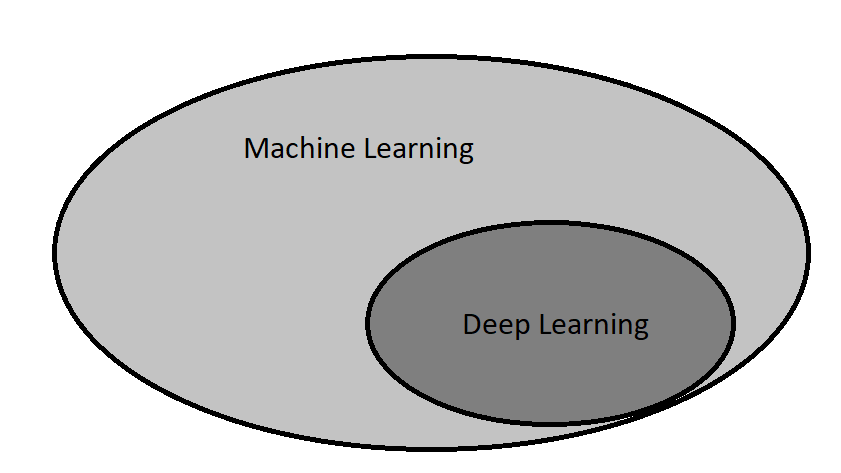
\includegraphics[width=8cm]{mldlunterschied.png}
  \caption{Abgrenzung Deep Learning zu Machine Learning}
  \label{dlmlunterschied}
\end{figure}

\subsection{Convolutional Neural Networks}

\textit{Convolutional Neural Networks} (CNN) sind eine spezielle Art von neuronalen Netzen, die sich für das verarbeiten von gitterartig beschaffenen Daten eignen. Hierzu zählen zum Beispiel auch Bilddaten, deren Pixelraster sich als Gitter oder Matrix interpretieren lassen. Ein typisches CNN besteht dabei aus einem oder mehreren Paaren von \textit{Convolutional}- und \textit{Pooling-Layern}, gefolgt von einem oder mehreren \textit{Fully-Connected-Layern}. Die Folgenden Darstellungen richten sich im wesentlichen nach Goodfellow \cite[S.326-366]{Goodfellow-et-al-2016}
\paragraph{Convolutional Layer}
Bei einem \textit{Convolutional Layer} wird schrittweise ein Filterkernel $K$ über eine Eingabematrix $I$ mit den Dimensionen $n$ und $m$ bewegt (Abb. \ref{cnns}). Der Input der folgenden Neuronen $S(i,j)$ berechnet sich dann aus einer Faltungsoperation der jeweils übereinanderliegenden Kernel- und Bildelemente (Gleichung \ref{convolution}). 
\begin{equation}\label{convolution}
	S(i,j)=(I\ast K)(i,j)=\sum_{n}\sum_{n} I(i-m,j-n)K(m,n)
\end{equation}
Der so berechnete Input eines Neurons wird anschließend abhängig von der verwendeten Aktivierungsfunkton in den Output verwandelt. Zu bemerken ist, dass alle Neuronen eines \textit{Convolutional Layers} die gleichen Gewichte haben (sog. \textit{Parameter Sharing}). Dadurch ist es möglich Speicher gegenüber anderen Netzstrukturen einzusparen, die häufig eine große Gewichtungsmatrix verwenden. Ein weiterer großer Vorteil sind die sog. \textit{Sparse Interarctions}. Durch die Verwendung eines Filterkernels der meist nur einen Bruchteil der Größe des zu analysierenden Bildes aufweist, werden nur die Features extrahiert, die wirklich entscheidend sind für die Zugehörigkeit zu einer Klasse. Dies führt ebenso zu einer weiteren Speicher- und Performanzoptimierung.
\begin{figure}[h!]
  \centering
  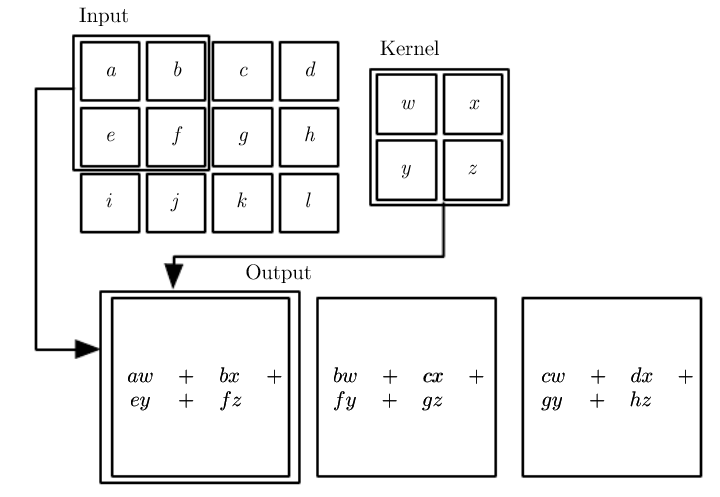
\includegraphics[width=12cm]{cnn_prinzip.png}
  \caption{Prinzip eines Convolutional Layers \cite[S.330]{Goodfellow-et-al-2016}}
  \label{cnns}
\end{figure}
\paragraph{Pooling Layer}

\textit{Pooling Layer} sorgen dafür, dass Features einer Klasse in einem Bild nahezu ortsinvariant gelernt werden können. Ein weitverbreitetes Pooling Verfahren ist das sog. $2X2$ \textit{Max-Pooling}, bei dem aus jedem $2X2$ Quadrat der Neuronen des \textit{Convolutional-Layers} nur das aktivste Neuron an die nächste Schicht weitergeleitet wird. Abbildung \ref{poolinglayer} verdeutlicht dieses Funktionsprinzip. Es werden von den jeweils benachbarten Neuronen nur die mit den höchsten Gewichten an die nächste Schicht durchgeschaltet.
\begin{figure}[!h]
  \centering
  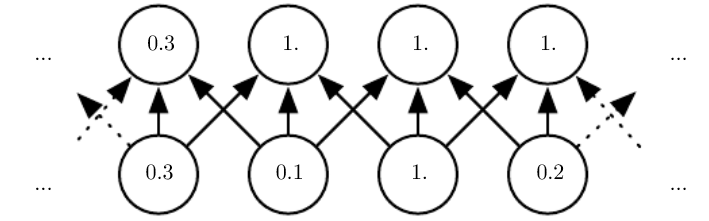
\includegraphics[width=12cm]{pooling_layer.png}
  \caption{Prinzip eines Pooling Layers \cite[S.337]{Goodfellow-et-al-2016}}
  \label{poolinglayer}
\end{figure} 
\FloatBarrier

\paragraph{Fully Connected Layer}

\textit{Fully-Connected-Layer} oder in \textit{Keras} sog. \textit{Dense-Layer} stellen einen Schichtentyp dar, bei dem jedes Neuron mit jeweils jedem Neuron der vorigen Schicht verschaltet ist. Es ist so möglich, die Ausgaben des letzten \textit{Pooling-Layers} über ein oder mehrere \textit{Fully-Connected-Layer} mithilfe von Aktivierungsfunktionen zum Beispiel in eine Wahrscheinlichkeitsverteilung der Klassenzugehörigkeit zu überführen. Die Anzahl Neuronen in der letzten Schicht entspricht dann der Anzahl zu lernender Klassen oder auch der Anzahl vorherzusagender Features.

\subsection{Loss-Funktionen und Metriken}

DL Netze optimieren ihre Gewichte und Neuronenaktivitäten während des Trainings selbst durch einen Vergleich der geschätzten Ergebnisse $y_{pred}$ mit den entsprechenden Zielgrößen $y_{target}$. Dies geschieht über sog. \textit{Loss-Functions}. Dabei zeigen diese Funktionen bei großen Abweichung von den Zielwertebereichen typischerweise auch hohe Werte \cite[S.271-279]{Goodfellow-et-al-2016}. Ein weit verbreitetes Beispiel hierfür ist der mittlere quadratische Fehler (\textit{Mean-Squared-Error (MSE)}), der häufig als Maß zur Evaluation des Trainingserfolges eingesetzt wird. Der MSE berechnet sich entsprechend Gleichung \ref{mse}. Die MSE-Loss-Funktion wird auch als L2-Loss bezeichnet. Diese Möglichkeit zur Beurteilung des Erfolges eines DL-Modells wird in Keras auch als Metrik bezeichnet. Als Metriken werden meist ebenso die beschriebenen Loss-Funktionen verwendet. Metriken haben einen rein informativen Zweck und werden nicht direkt für das Training verwendet \cite{chollet2015keras}. Loss-Funktionen spiegeln so einen entscheidenden Faktor für ein erfolgreiches Training wieder. Dabei sollte je nach Anwendungsfall individuell eine passende und sinnvolle Loss-Funktion zur Validierung gewählt werden. Ein ausführliche Abhandlung hierüber findet sich in \cite{dlbook2018} und \citep{dlazure2019}.
\begin{equation}\label{mse}
	MSE=\sum_{n} \frac{(y_{pred}-y_{target})^2}{n}
\end{equation}

\subsection{Stand der Technik}

In der Literatur werden viele Möglichkeiten zur Objekterkennung mittels DL beschrieben. Laut Zhao haben sich aktuell jedoch drei Hauptverfahren in der Industrie etabliert \cite{Detection2019}. \textit{Fast-Region-Based-CNNs} ermöglichen gute Detektionsergebnisse, sind aber relativ rechenaufwendig \cite{Girshick2015}. Das \textit{You Only Look Once} Modell (YOLO) erreicht eine höhere Performanz bei verbesserter Präzision \cite{Redmon2016}. Ein weiteres Modell zur Lösung des Problems ist das von Liu vorgestellte \textit{Single-Shot-Detection} (SSD) Modell vor. Beim SSD können Performanz und Genauigkeit zu Lasten einer komplexeren Netzarchitektur noch weiter verbessert werden \cite{Liu2016}. Die Gemeinsamkeit aller vorgestellten Modelle besteht in der Verwendung von \textit{Convolutional Layern}.

\section{Methoden}

Zu Lösung der Aufgabenstellung wird die sogenannte YOLO (\textit{You Only Look Once}) Netzstruktur in Python unter Nutzung der Keras API implementiert. YOLO Netze zeichnen sich durch gute Detektionsergebnisse bei einer sehr hohen Trainings- und Klassifikationsperfomanz aus. So ist mithilfe des YOLO-Modells sogar auf vergleichsweise kostengünstiger Hardware eine Echtzeitschätzung der Bounding-Boxen von Objekten möglich \cite{Redmon2016}. 

\subsection{Lossberechnung und Intersection over Union}
\label{Loss_ber}
Rezatofighi1 beschreibt die \textit{Intersection over Union} (IOU) als eine performante und präzise Möglichkeit den Loss bei der Objekterkennung zu bestimmen (s. Kap 2.2). Dabei wird die IOU aus dem Quotienten der sich überlappenden Fläche \textit{(Intersection / Overlap)} und der gemeinsam gebildeten Fläche (\textit{Union}) zweier Regionen berechnet: 
\begin{equation}\label{iou}
	IOU(y_{target},y_{pred})=\frac{y_{target} \cap y_{pred}}{y_{target} \cup y_{pred}}
\end{equation}
$y_{pred}$ steht hierbei für die geschätzte und $y_{target}$ für die reale Bounding-Box der Objekte. Die graphische Interpretation der Berechnung wird in Abbildung \ref{ioubild} deutlich. Zur Berechnung der jeweiligen Flächen wird der von Rezatofighil in \cite{Rezatofighi1902} beschriebene Algorithmus implementiert. Dort ist zusätzlich eine hier nicht genutzte Erweiterung zur \textit{Generalized-IOU} beschrieben.
\begin{figure}[!h]
  \centering
  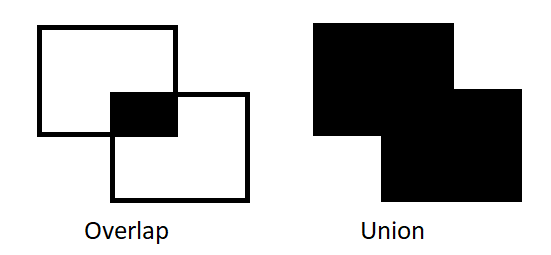
\includegraphics[width=8cm]{iou.png}
  \caption{Intersection over Union}
  \label{ioubild}
\end{figure} 
\FloatBarrier
Somit ergibt sich für den 2D-Fall als resultierende Loss-Funktion:
\begin{equation}\label{iouloss}
	L_{2D}= 1-IOU(y_{target},y_{pred})
\end{equation} 
Es ist darauf hinzuweisen, dass aufgrund der hohen Komplexität auf die Erweiterung der IOU Berechung für den 3D-Fall im Rahmen dieser Arbeit verzichtet wird. Möglich Ansätze für 3D-IOU Berechungen finden sich jedoch in \cite{Xu2019} und \cite{Mousavian1612}. Im 3D-Fall wird der Loss lediglich über den in Kapitel 2.2. beschriebenen L2-Ansatz bestimmt. In Abbildung \ref{L2_loss_graphik} ist schematisch dargestellt wie der L2 Loss berechnet wird. Hierfür wird lediglich der Abstand zwischen einem, vom Netz prädizierten Punkt und einem Zielpunkt berechnet. Dieser Abstand etspricht dem Ausdruck $y_{target}-y_{pred}$ aus Formel \ref{mse}. 
\begin{figure}[!htb]
  \centering
  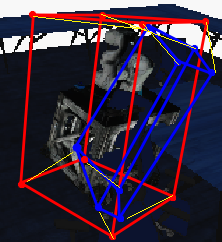
\includegraphics[width=6.2cm]{Abb/l2_loss_bei3d_bb.png}
  \caption{Prädizierte und gelabelte Bpounding}
  \label{L2_loss_graphik}
\end{figure} 
\newpage
\subsection{Netzstruktur}

\begin{figure}[!htb]
  \centering
  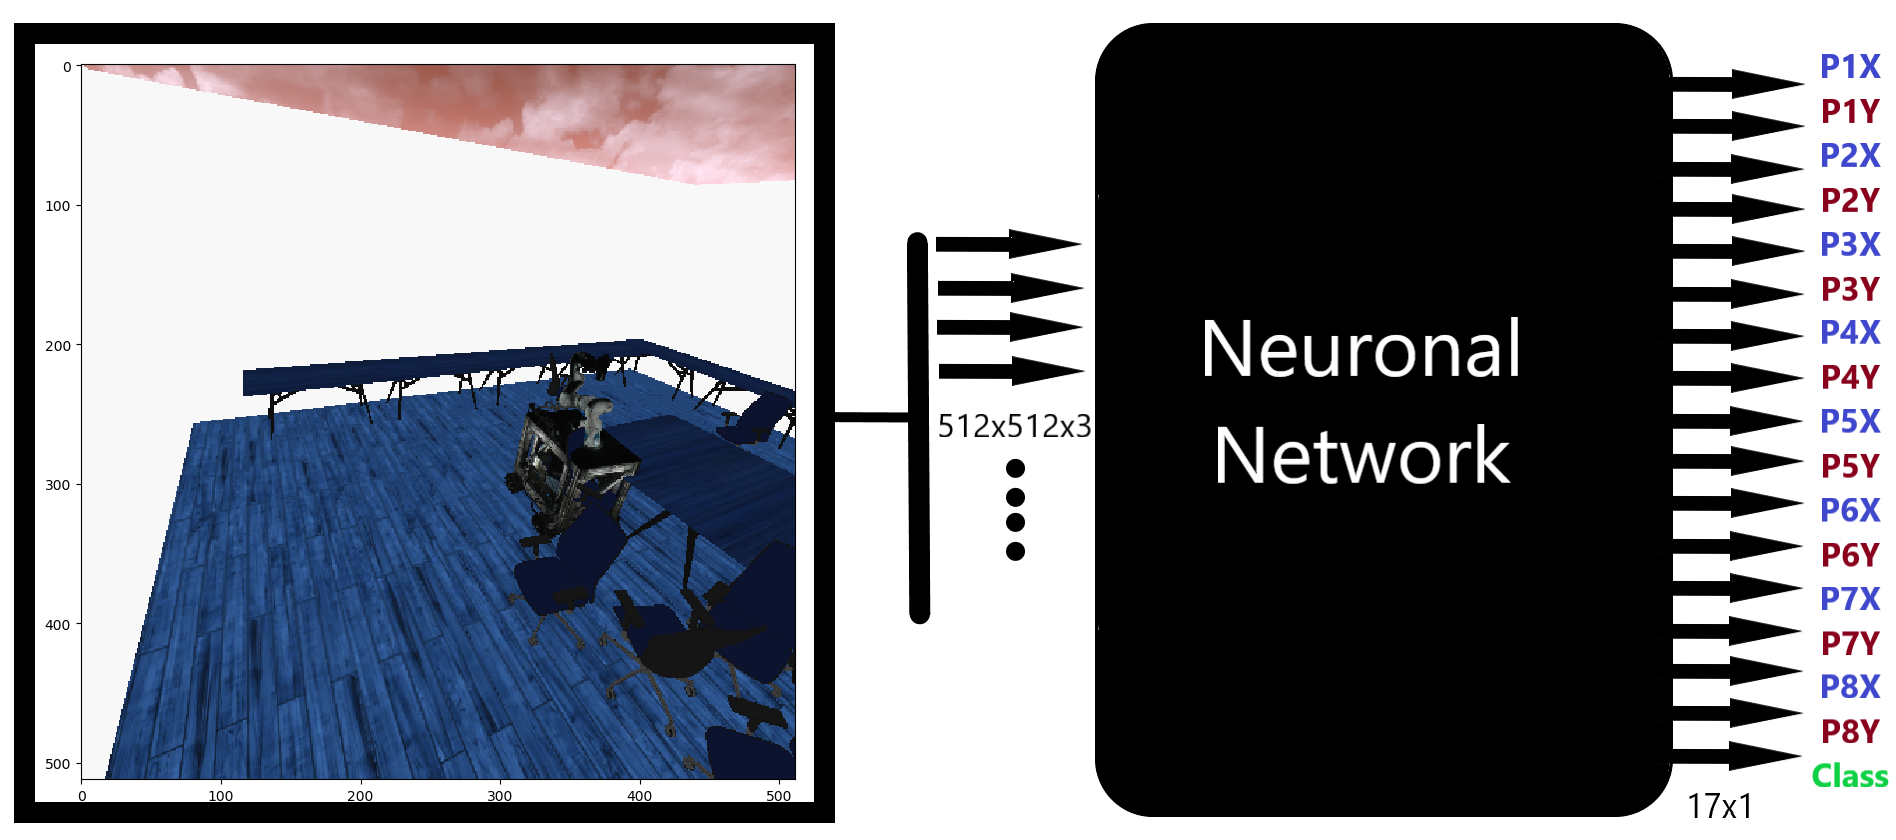
\includegraphics[width=13.8cm]{Abb/Modell_struktur.png}
  \caption{Grobe Darstellung der Netzstruktur zur prädiktion einer 3D Bounding-Box}
  \label{grobe_netz_struktur}
\end{figure} 

Die Netzstruktur, welche für die prädiktion einer 3D Bounding-Box verwendet wird orientiert sich sehr stark an dem sogenannten YOLO Netz. Die ersten Schichten des Netzes bestehen aus \textit{convolutional layern}, welche die Aufgabe haben Features aus dem Bild zu extrahieren. Die hintere Schicht des Netzes besteht aus  \textit{fully connected layern}, welche die Koordinaten der Bounding-Box Punkte sowie die Klassenzugehörigkeit  ausgeben \cite{Redmon2016}. \\Die Netzarchitektur muss jedoch für die Prädiktion einer projizierten 3D Bounding-Box angepasst werden. Diese besitzt im gegensatz zu einer 2D Bounding-Box 8 anstatt 2 erforderlichen Bildpunkten. Eine Vergleich einer 2D und einer 3D Bounding-Box ist in Abbildung \ref{3D_Bounding_roboter} aufgezeigt. Aus den 8 Punkten ergeben sich 16 Koordinaten. Zu den 16 Koordinaten kommt eine weitere Angabe über die Klasse des Objekts. Diese Angabe wird nur deshalb implementiert, um das Netz modularer und skalierbarer zu  machen. In dem hier behandelten Fall gibt es allerdings nur die eine Klasse namens \textit{Roboter}. in Abbildung \ref{grobe_netz_struktur} ist eine grobe Darstellung des implementierten Netzes als Blackbox dargestellt. Zu sehen sind die 17 Ausgänge, welche aus 16 Koordinaten für die Punkte der 3D Bounding-Box, sowie der Klassenzugehörigkeit bestehen. Im Anhang in Abbildung ... ist das Verwendete Netz detailliert dargestellt.

\begin{figure}[!htb]
  \centering
  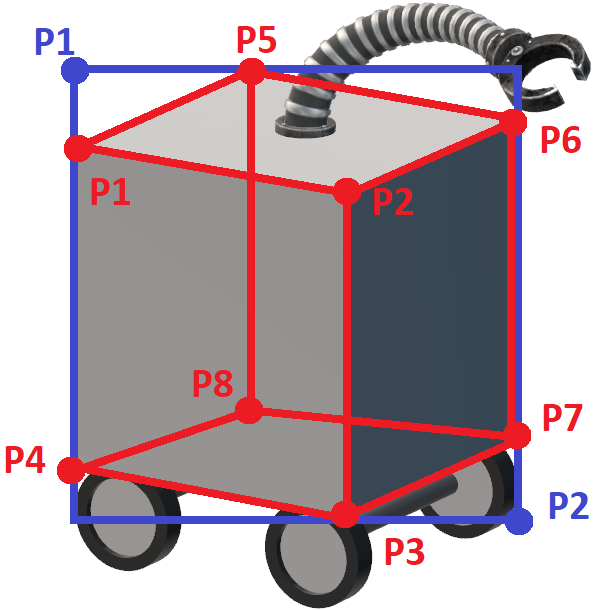
\includegraphics[width=6.8cm]{Abb/3d_robotter_mit_boundig_box_2d_vs_3d.PNG}
  \caption{3D Bounding-Box mit 8 Punkten \textcolor{red}{(rot)} und im Vergleich dazu eine 2D Bounding-Box mit 2 Punkten \textcolor{blue}{(blau)} }
  \label{3D_Bounding_roboter}
\end{figure} 

\newpage
\subsection{Training}
Für das Training wird ein gelabelter Datensatz verwendet, welcher vom Institut für eingebettete Systeme und Medizintechnik der Hochschule Mannheim bereitgestellt wird. Es liegen insgesamt 1000 gelabelte Samples vor, von denen 90\% für das Training und 10\% für die Validierung verwendet werden. Alle weiteren Trainingsparameter sind Tabelle \ref{trainings_param} zu entnehmen.\\

\begin{table}[!htb]

\centering
\caption{Trainingsparameter}
\begin{tabular}{ll}
\label{trainings_param}
\textbf{Parameters}                  & \textbf{Values} \\ \hline
\\Convolutional Layer        & 9      \\
Fully connected Layer       & 2      \\
Anzahl der Trainingssamples & 900    \\
Epochen                  & 15     \\
Batch Size                  & 1     \\
Optimizer                   & Adam   \\
Learning Rate               & 0,0001 \\
Loss Function               & MSE (siehe \ref{Loss_ber})   
\end{tabular}
\end{table}
Auf einer NVIDIA GTX9600M Grafikkarte mit mit einer \textit{NVIDIA Compute Capability} von 5, benötigt das Training des Netzwerks zur Detektion einer 3D Bouding box lediglich 12 Minuten.
  
\subsection{Softwaremodul Beschreibung}
Für die Realisierung eines Netzwerkes zu Bestimmung einer 3D Bounding-Box werden einige Softwaremodule implementiert. Im folgenden werden diese Module beschrieben. 
\subsubsection{Laden der Daten}
Das laden der Trainingsdaten wird durch eine eigens dafür entwickelte klasse Implementiert. Die Bilder liegen im .png Format und die Labls im .json Format vor. Die Klasse lädt diese Daten, teilt diese in Trainings- und Testdaten auf und gibt die Daten als \textit{numpy arrays} zurück, sodass diese direkt für das Training verwendet werden können. In Abbildung \ref{UML_load} ist das zu der Klasse gehörige UML Diagramm mit allen Methoden aufgezeigt.
\begin{figure}[!htb]
  \centering
  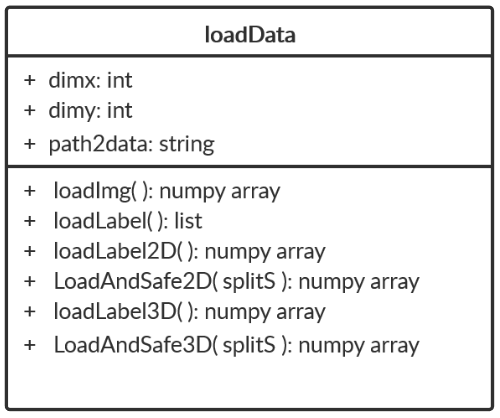
\includegraphics[width=6.8cm]{Abb/ULM_class_loadData.PNG}
  \caption{UML Diagramm loadData}
  \label{UML_load}
\end{figure} 
\subsubsection{Objekt Lokalisierung}
in der Klasse \textit{ObjectLocalizer3D} befindet sich der für das Neuronale Netz relevante Programmcode. Hier wird unter anderem das Netz erzeugt, die Loss Funktion definiert, sowie eine Metrik geschrieben. Die Klasse ist abgeleitet von der \textit{Keras functional API}. Die Klasse besitzt auch Methoden, wie fit, welche direkt auf die zu der \textit{Keras functional API} zugehörige fit Methode zugreift. Ebenfalls ist es möglich die Trainierten Modelle zu speichern oder diese zu Laden. In Abbildung \ref{UML_localizer} ist ein UML Diagramm der Klasse dargestellt.  
\begin{figure}[!htb]
  \centering
  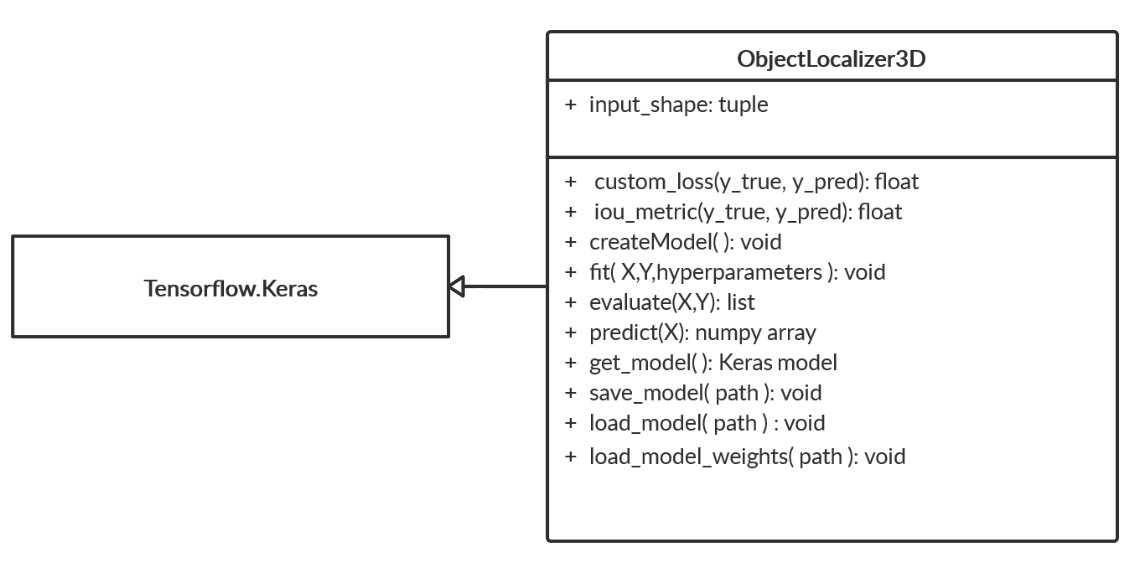
\includegraphics[width=13.8cm]{Abb/ULM_class_objectLocalizer.PNG}
  \caption{UML Diagramm der Klasse ObjectLocalizer3D, welche von der \textit{Keras functional API} abgeleitet ist}
  \label{UML_localizer}
\end{figure} 
\newpage

   

\section{Ergebnisse}

Die in Abschnitt 3.2 beschriebene Netzstruktur wird mit dem in Abschnitt 3.3 vorgestelltem Datensatz und Parametern trainiert und validiert. Die optimalen Trainingsparameter wurden dabei aus mehren Experimenten empirisch ermittelt. Dabei dient die in Abschnitt 3.1 erarbeitete \textit{Loss}-Metrik zur jeweiligen Quantisierung des Trainingserfolges. \\Abbildung \ref{lossbild} zeigt den Verlauf des \textit{Loss} jeweils für die Trainings- und Validationsdaten über die Trainingsepochen im 3D-Fall. Dabei fällt dieser zunächst relativ schnell und nähert sich dann ungefähr $1*10^{-3}$ an. Dies deutet auf ein erfolgreiches Training ohne \textit{Overfitting} hin. In Abbildung 11 und 12 werden beispielhaft zwei prädizierte Bounding-Boxen der Testdaten dargestellt (blau). Zum Vergleich sind zusätzlich die manuell vorgelabelten Bounding-Boxen eingezeichnet (rot). Oben im Bild steht der jeweils errechnete \textit{Loss}. Es ist zu erkennen, dass das rechte Bild mit dem höchsten \textit{Loss} auch die sichtbar größte Abweichung der prädizierten Bounding-Box mit der vorgelabelten aufweist. Der \textit{Loss} im linken Bild ist relativ gering und spiegelt so auch die sichtbar geringe örtliche Abweichung der prädizierten Bounding-Box zur vorgelabelten Bounding-Box wieder.\\ 
 
\begin{figure}[!htb] 
  \centering
  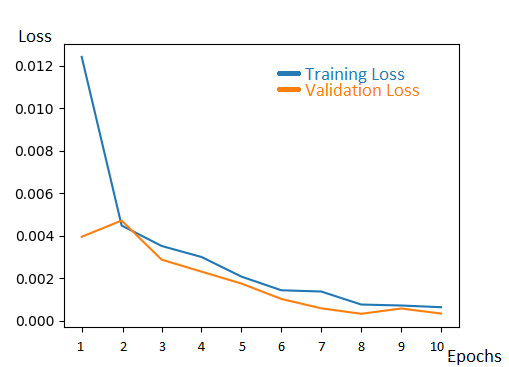
\includegraphics[width=13.8cm]{Abb/training_progress.png}
  \caption{Trainings- und Validations-Loss über die Trainingsepochen}
  \label{lossbild}
\end{figure} 
 \label{pred_boxes}
\begin{figure}[!htb]
   \begin{minipage}[b]{.5\linewidth} % [b] => Ausrichtung an \caption
      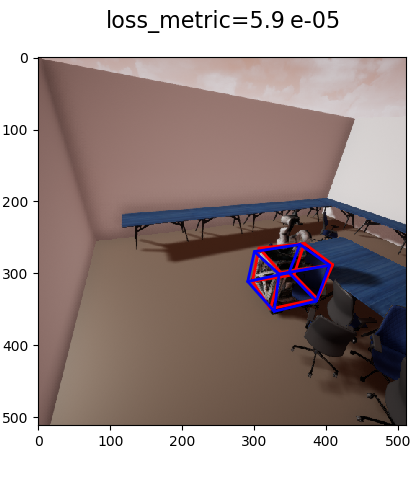
\includegraphics[width=\linewidth]{bbs/gut.png}  
      \label{tiv_ausgang}    
      \caption{Beispiel einer gut prädizierten Bounding-Box mit geringem Loss. Zu sehen ist die gelabelte Bounding-Box (rot), sowie die prädizierte Bounding-Box (blau).}
   \end{minipage}
   \hspace{.03\linewidth}% Abstand zwischen Bilder
   \begin{minipage}[b]{.5\linewidth} % [b] => Ausrichtung an \caption
      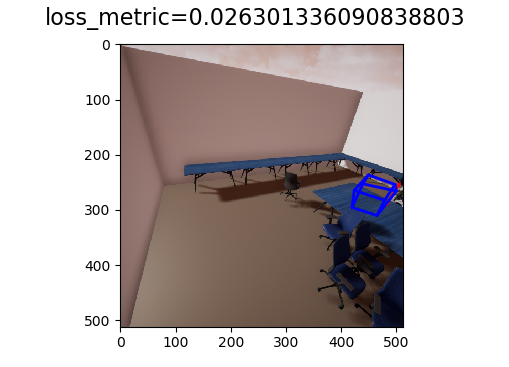
\includegraphics[width=\linewidth]{bbs/schlecht.png}
      \label{vdiffX_unsymm} 
      \caption{Beispiel einer schlecht prädizierten Bounding-Box mit hohem Loss. Hier könnte speziell der Stuhl die Schätzung negativ beeinflusst haben.}
   \end{minipage}
\end{figure}
\newpage
\newpage
\section{Fazit und Ausblick}

In der vorliegenden Arbeit wurde erfolgreich ein \textit{Deep-Learning} Netzwerk zur Detektion einer 3D Bounding-Box trainiert und validiert. Als Netzstrukur dient dabei eine modifizierte Version des \textit{YOLO}-Netzes. Zur Validierung im 2D-Fall dient die \textit{IOU}-Metrik. Im 3D-Fall wird der \textit{Loss} mittels der L2-Metrik ermittelt. Die optimalen Hyperparameter sind empirisch aus verschiedenen Experimenten hervorgegangen.
Zusätzlich ergeben sich vielversprechende Anknüpfungspunkte für weitere Arbeiten. Atiqur beschreibt zum Beispiel eine Möglichkeit die IOU Berechung im 2D-Fall noch weiter zu optimieren in \cite{Atiqur}. Weiterhin wäre es interessant die IOU auch für die Berechnung der Loss Funktion im 3D Fall zu benutzten. Möglich Ansätze für 3D-IOU Berechungen finden sich in \cite{Xu2019} und \cite{Mousavian1612}. Eine weitere Möglichkeit zur Verbesserung der Trainingsergebnisse liegt in der Augmentation der Daten. Darauf wird im Rahmen dieser Arbeit jedoch verzichtet.


\section{Literatur und Bilder}

\bibliographystyle{plain}
\bibliography{dlm_doku_literature}
\listoffigures


\end{document}
